\documentclass{beamer}
\usepackage{amsthm}
\usepackage{amsmath,amssymb}
\usepackage{graphicx}
\usepackage{lmodern}
\usepackage[T1]{fontenc}
\usepackage{tikz}
\usetikzlibrary{decorations.markings}

\tikzstyle{every node}=[circle, draw, fill=black!50, inner sep=0pt, minimum width=4pt]
\tikzset{->-/.style={decoration={
      markings,
      mark=at position .5 with {\arrow{>}}},postaction={decorate}}}
\tikzset{-<-/.style={decoration={
      markings,
      mark=at position .5 with {\arrow{<}}},postaction={decorate}}}

\newtheorem{conjecture}{Conjecture}
\newtheorem*{prop}{Proposition}
\newtheorem*{defin}{Definition}

\title{Week 5 Presentation}
\author{Max Comstock}
\date{Summer 2014}

\begin{document}

\frame{\titlepage}

\begin{frame}
\frametitle{Recall: Encoding graphs as polynomials}
\begin{prop}
  Let $G = (V,A)$ be a simple directed graph on vertices $V = \{1, \ldots, n\}$. Assume that the characteristic of $\mathbb{K}$ is relatively prime to $n$ and that $z \in \mathbb{K}$ is a primitive $n$-th root of unity. Consider the following system in $\mathbb{K}[x_1, \ldots, x_n]$:
  \begin{align*}
    H_G = \{x_i^n - 1 = 0, \prod_{j \in \delta^+(i)} (z x_i - x_j) = 0 \, : \, i \in V\}
  \end{align*}
  Here, $\delta^+(i)$ denotes those vertices $j$ which are connected to $i$ by the arc going from $i$ to $j$ in $G$. The system $H$ has a solution over $\mathbb{K}$ if and only if $G$ has a Hamiltonian cycle.
\end{prop}
Source: ``Recognizing Graph Theoretic Properties with Polynomial Ideals'' by J.A. De Loera, C. Hillar, P.N. Malkin, and M. Omar.
\end{frame}

\begin{frame}
\frametitle{Recall: Graphs with one Hamiltonian cycle}
\begin{defin}
  Let $z$ be a fixed primitive $k$-th root of unity. If $C$ is a directed cycle of length $k$ in a directed graph, with vertex set $\{v_1, \ldots, v_k\}$, the cycle encoding of $C$ is the following set of $k$ polynomials:
  \begin{align*}
    g_i = \left \{ \begin{matrix} x_{v_{k-i}} - z^{k-i} x_{v_k} & i = 1, \ldots, k-1\\ x_{v_k}^k - 1 & i = k \end{matrix} \right ..
  \end{align*}
\end{defin}
Note: define $H_{G,C} = \langle g_1, \ldots, g_i \rangle$. The $g_i$'s form a reduced Gr\"obner basis (which must be unique) for $H_{G,C}$.
\end{frame}

\begin{frame}
\frametitle{Example}
The graph
\begin{center}
  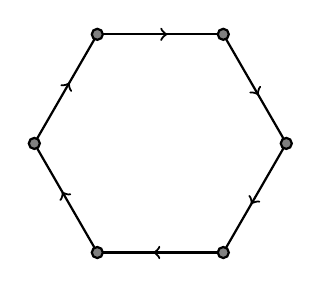
\begin{tikzpicture}[thick,scale=0.4]
    \draw[-<-] (0,0) -- (4,0);
    \draw[-<-] (4,0) node{} -- ++(60:4);
    \draw[-<-] (4,0)++(60:4) node{} -- ++(2*60:4);
    \draw[-<-] (4,0)++(60:4)++(2*60:4) node{} -- ++(3*60:4);
    \draw[-<-] (4,0)++(60:4)++(2*60:4)++(3*60:4) node{} -- ++(4*60:4);
    \draw[-<-] (4,0)++(60:4)++(2*60:4)++(3*60:4)++(4*60:4) node{} -- (0,0) node{};
  \end{tikzpicture}
\end{center}
gives us the following Gr\"obner basis for $H_G$:
\begin{align*}
	\{x_6^6-1, x_5-x_6z^5, x_4-x_6z^4, x_3-x_6z^3, x_2-x_6z^2, x_1-x_6z\}.
\end{align*}
\end{frame}

\begin{frame}
\frametitle{Example with two Hamiltonian cycles}
The graph
\begin{center}
  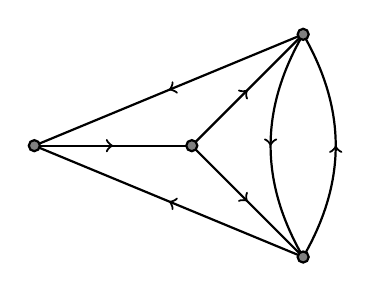
\begin{tikzpicture}[thick, scale=0.5]
    \path (4,0)++(45:4) coordinate(upper);
    \path (4,0)++(-45:4) coordinate(lower);
    \draw[->-] (upper) to (0,0);
    \draw[->-] (lower) to (0,0);
    \draw[->-] (upper) to[bend right] (lower);
    \draw[->-] (lower) to[bend right] (upper);
    \draw[->-] (0,0) node{} to (4,0);
    \draw[->-] (4,0) to ++(45:4) node{};
    \draw[->-] (4,0) node{} to ++(-45:4) node{};
  \end{tikzpicture}
\end{center}
has two Hamiltonian cycles. The Gr\"obner basis for $H_G$ is
\begin{align*}
	\{& x_4^4-1, x_3^2+x_4^2, 2x_2+(z+1)x_3+(z+1)x_4,\\& 2x_1+(-z+1)x_3+(-z+1)x_4\}.
\end{align*}
\end{frame}

\begin{frame}
\frametitle{Conjectures}
\begin{conjecture}
	For a graph $G$ with $n$ vertices and one or more Hamiltonian cycles, we find $x_n^n - 1 \in H_G$.
\end{conjecture}
\begin{conjecture}
	Let $G$ be a graph with $n$ vertices and one or more Hamiltonian cycles, and $k$ be a natural number (not including zero). Then we find, for each $i$ such that $1 \leq i \leq n$, that $\mathrm{LT}(g) = x_i^k$ for some $g \in H_G$.
\end{conjecture}
\begin{conjecture}
	Let $G$ be a graph with $n$ vertices, and $k \geq 2$. There exists $g \in H_G$ such that $\mathrm{LT}(g) = x_i^k$ for some $i$ such that $1 \leq i < n$ if and only if $G$ has more than one Hamiltonian cycle.
\end{conjecture}
\end{frame}


\end{document}
